%########################################################################################
% Chapter: Wissen in synchronen und asynchronen Systemen
%########################################################################################
\section{Wissen in synchronen und asynchronen Systemen}
\label{sync_vs_async}
%\begin{figure}[H]
%\centering
%      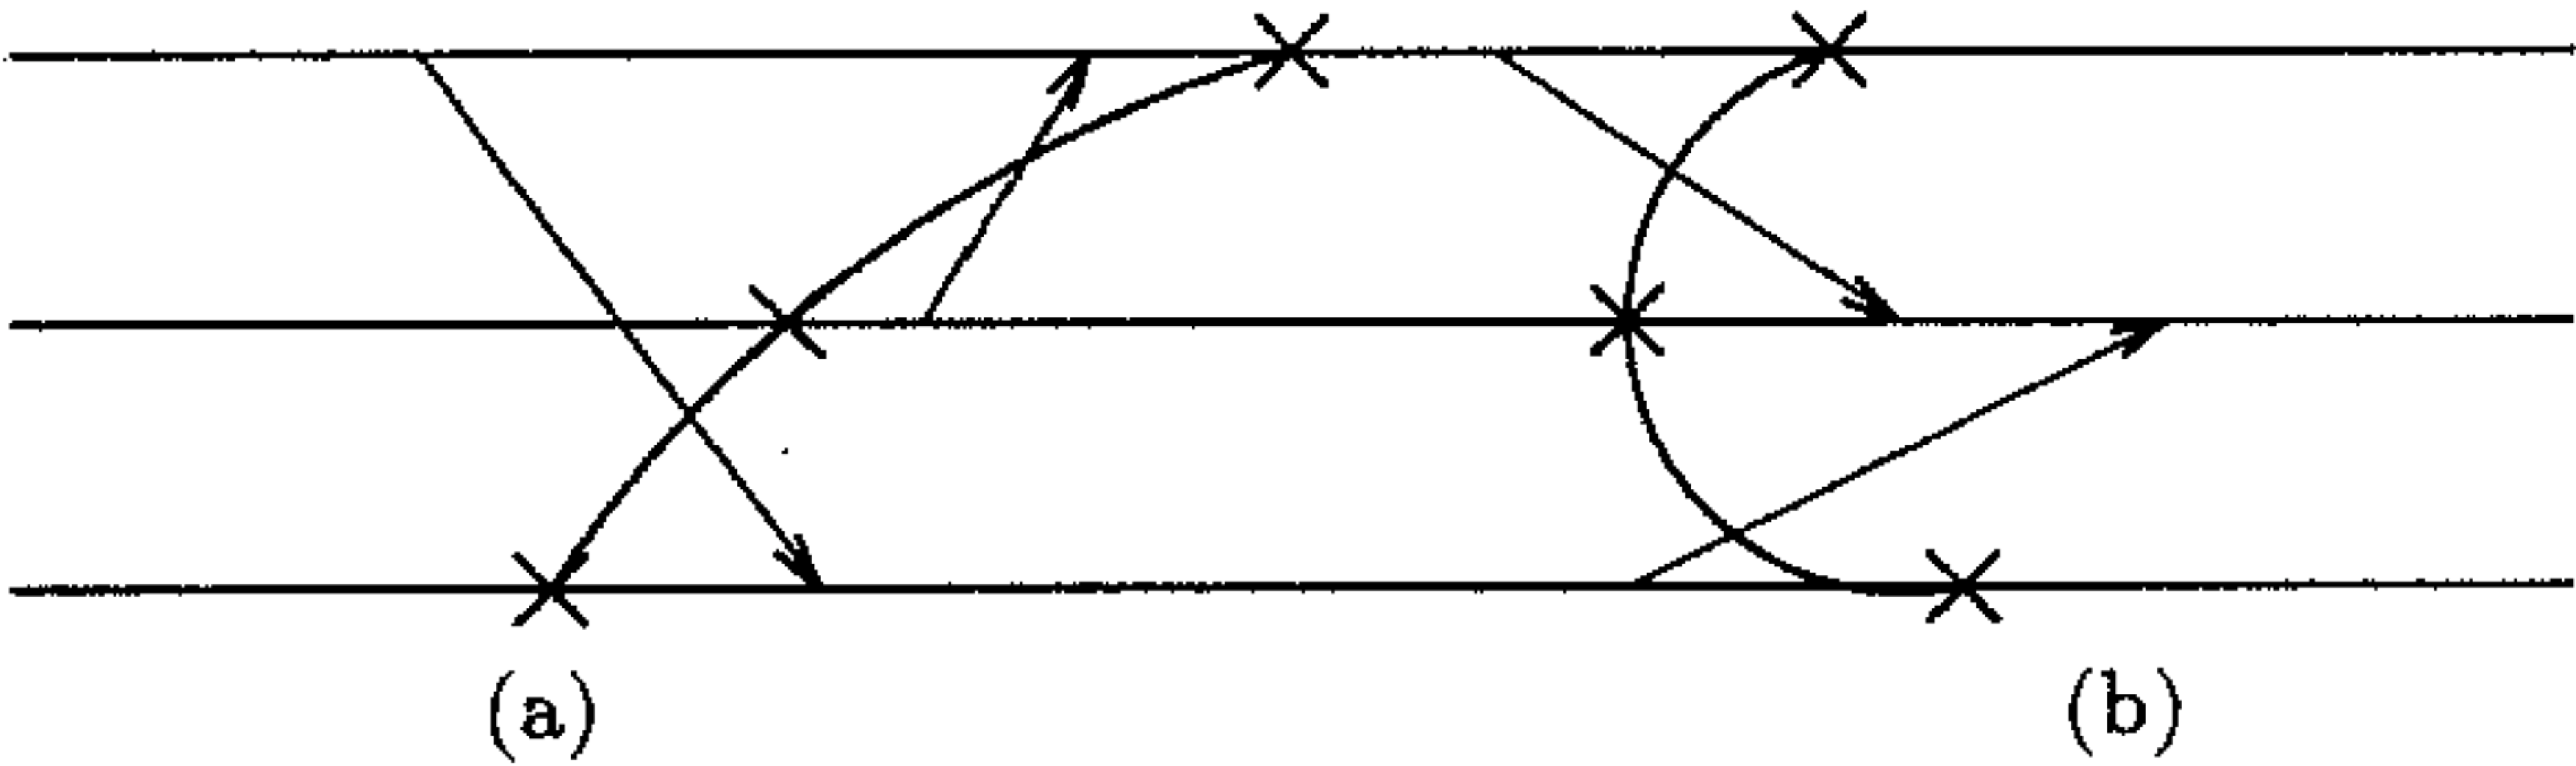
\includegraphics[width=0.8\textwidth]{def_async_sys.pdf}
%  \caption{ \cite{Panangaden1992} }
%\label{pic:fismahistorical}
%\end{figure}
Nachfolgend wird in diesem Kapitel beispielhaft erläutert, wie die Problematik des \textit{cheating husbands}-Rätsel für die Fälle der asynchronen und synchronen Übertragung behandelt werden.

%########################################################################################
% Section: Wissen in asynchronen Systemen
%########################################################################################
\subsection{Wissen in asynchronen Systemen}
\label{wissen_sync}
Für die asynchronen Systeme gibt es einen Zusatz in dem Rätsel der \textit{cheating husbands} (\cite{moses1986cheating} et al.). Es beginnt damit, dass Henrietta I verstirbt und damit ihre Tochter (Henrietta II) die Herrschaft von Mamajorca übernimmt. Der letzte Wunsch ihrer Mutter war es, dass Benachrichtigungssystem für betrogene Ehefrauen fortzuführen. \\\\
Die Tochter kam der Bitte ihrer Mutter nach. Jedoch vollführte sie eine Verbesserung des Systems. Um die Kommunikation zu erleichtern lies Henrietta II Briefkästen an jedem Haushalt in der ganzen Stadt anbringen. Danach lies die Königin als erstes einen Brief an alle ausliefern, in dem die Neuerungen erläutert wurden und die Eigenschaften des neuen Systems veranschaulicht wurden. Die erste Eigenschaft besagt, dass jeder Brief den die Königin verschickt garantiert, zu einem \textit{nicht vorhersagbaren Zeitpunkt}, eine der Frauen erreichen wird. Die zweite Eigenschaft ist  ableitbar aus der Ersten. Sie besagt lediglich, dass keine Ankündigungen mehr auf dem Marktplatz gemacht werden müssen.\\\\
Der grundsätzliche Gedanke ist der gleiche. D.h. nach Erhalt der Nachricht wird der untreue Ehemann in der folgenden Nacht erschossen. Aufgrund des zeitversetzten Zustellens der Nachricht gibt es Zustände in einem System, welche nicht vorhersagbar sind. Jenes Problem wird nachfolgend im Theorem \ref{theo_async_1} erläutert.
\begin{theorem}[vgl. Theorem 2, \cite{moses1986cheating} S. 170]\\
\label{theo_async_1}
Wenn mehr als ein untreuer Ehemann existiert und die Nachricht wird über einen asynchronen Kanal verteilt, so stirbt kein Ehemann erschossen.
\end{theorem}
\begin{proof}
Der Beweis ist durch Veranschaulichung des Ablaufs leicht zu erbringen. Durch die asynchrone Verteilung der Briefe und die Tatsache, dass es eine eventuelle Verteilung dieser Briefe gibt handelt es sich um "'eventual common knowledge"' (siehe Kap. \ref{GemeinsamesWissen}). Wird nun ein Brief von der Königin versendet, erhält jede Frau eventuell den Brief, der für sie bestimmt war und die besagt Frau weiß ebenfalls, dass es eventuell noch weitere Fr%nauen gibt, die einen Brief erhalten haben könnten. Es gibt keine Sicherheit für die Frauen, ob ihr Ehemann zweifelsfrei einer der untreuen ist. Zweifelsfrei kann sich dies deshalb nicht sagen lassen, da die Frau nicht weiß, ob die ruhigen Nächte auf der Tatsache basieren, dass die anderen Briefe noch nicht zugestellt wurden oder ob es eine Reaktion andere Frauen auf den Erhalt eines Briefes ist.%$\square$%
\end{proof}
Aus dem Beweis resultiert, dass sich die Frauen aufgrund der Unsicherheit nie dazu entschließen würden, ihren Gemahlen zu erschießen, denn es könnte sich ja auch um einen Irrtum handeln, da noch nicht alle Briefe zugestellt wurden.\\\\
Dieses Verhalten lässt sich auf verteiltes Wissen übertragen. Mit diesem Ansatz ohne jegliche Verbesserungen, wie bereits vorgestellt, kann in asynchron verteilten Systemen nicht festgestellt werden, ob die Nachricht angekommen ist oder nicht. Es operiert nach dem Prinzip "'Fire and Forget"'. Dies bedeutet, dass die Nachricht gesendet wird und was im Anschluss mit der Nachricht passiert, d.h. ob diese beim Kommunikationspartner ankommt oder verloren geht, spielt für den Sender keine Rolle mehr.$\square$\\\\
Für einen Ansatz mit asynchronen Systemen, in welchem es eine Bestätigung bzw. Quittung auf den Erhalt der Nachricht gibt, befassen sich auch andere Darstellungen. Eine von ihnen ist das Problem der byzantinischen Generäle. Hierbei sollen sich zwei räumlich getrennte Generäle durch das Aussenden eines Boten abstimmen, um gemeinsam eine im Tal liegende Armee anzugreifen. Dieser Bote muss allerdings durch das Tal, in welchem sich die feindlich gesinnte Armee befindet. Durch diesen Umstand kann diese Nachricht, ebenfalls verloren oder durch eine falsche Nachricht mittels eines Boten von der anzugreifenden Armee ersetzt werden. Gesetzt dem Fall, dass der Bote nicht abgefangen wird, so erhält der Bote eine Quittierung über den Erhalt der Nachricht und wird auf den Rückweg ausgesendet. Der General quittiert wiederum die Nachricht, dass er die Bestätigung seines Kollegen erhalten hat. Hierbei lässt sich leicht ausmachen, dass es schnell in einen endlosen Kreis der Bestätigung enden kann. Somit ist es in asynchron verteilten Systemen auch nicht allein mit dem Senden von Bestätigungen getan. Diese würden zu viel Belegung der Kanäle nach sich ziehen.


%########################################################################################
% Section: Wissen in synchronen Systemen
%########################################################################################

\subsection{Wissen in synchronen Systemen}
\label{wissen_sync}
Die Thematik von Wissen in synchronen Systemen kann in zwei Bereiche unterteilt werden. Zum einen in schwache, zum anderen in starke synchrone Systeme. In beiden Bereichen, wird wieder die Erzählung der "'cheating Husbands"' aufgegriffen und ausgebaut.
\subsubsection{Schwache synchrone Systeme}
\label{schwach_sync_wissen}
Bei schwachen synchronen Systemen wird zunächst gewährleistet, dass jeder Kommunikationsteilnehmer die Nachricht erhält. Wie dieser Mechanismus ausgeführt werden kann, wird im Nachgang aufgezeigt (Vgl. \cite{moses1986cheating} S. 170-171).\\\\
In der Geschichte wird Henrietta II von Henrietta III beerbt. Diese will ebenfalls das Benachrichtigungssystem fortführen. Wie ihre beiden Vorgängerinnen hat auch Henrietta III eine Idee wie das bisherige System verbessert werden könnte. Diese Verbesserung sieht vor, dass jeder Brief innerhalb einer gesetzten Grenze von b Tagen ihr Ziel erreicht. Für das Festlegen einer Grenze b wird von den Autoren der Begriff des „b-common-knowledge“ eingeführt. Es sagt aus, dass innerhalb von b Tagen jede Frau über das gleiche Wissen verfügt.\\\\
Für schwache synchrone Systeme führen die Autoren mehrere Annahmen ein, welche auch bewiesen werden. In dieser Ausarbeitung wird sich mit der Grundannahme auseinandergesetzt. Die weiterführenden Annahmen können in (\cite{moses1986cheating} S. 170-171) nachgeschlagen werden.

\begin{satz} [vgl. Proposition 3, \cite{moses1986cheating} S. 170-171]
\label{prop_weak_sync}
In schwachen synchronen Systemen mit einer Grenze b beim Ausliefern der Briefe, weiß eine Frau exakt von k untreuen Ehemännern, wenn $k \cdot b$ stille Nächte nach dem Erhalt des Briefes vorübergegangen sind.
\end{satz}
\begin{proof}\hfill\\
Im Ausgangszustand weiß eine Frau von keinen untreuen Ehemännern (k=0). Nach $k \cdot b=0$ leisen Nächten kann besagte Ehefrau den Rückschluss führen, dass ihr Ehemann untreu ist. Durch den letzten Brief der aktuellen Königin weiß die Frau nicht vorher, dass ihr Mann untreu war. \\Es kann nun angenommen werden, dass eine Frau von k untreuen Ehemännern weiß. Um feststellen zu können, dass ihr eigener Ehemann Untreu ist müssen $k \cdot b$ ruhige Nächte vorangegangen sein. Wenn eine Frau weiß, dass Ihr Mann treu ist, dann weiß jede betrogene Frau von k untreuen Männern, welche durch Induktion nacheinander ihren Mann erschießen, wenn $k \cdot b$ stille Nächte, nach Erhalt des Briefes, vorangegangen sind.\\ Wenn eine Frau weiß, dass ihr Ehemann treu ist und die erste betrogene Frau einen Brief einen Tag zuvor (b-1) erhält, so ist es möglich, dass keine Schüsse vor der $(k+1)b^{th}$ Nacht, nach Erhalt des Briefes fallen. So weiß die Frau mit der Annahme ihr Mann wäre treu, dass er dies doch nicht ist.
$\square$
\end{proof}
Es wird in diesem Zusammenhang von einem schwachen synchronen System gesprochen, da es durchaus noch zu Zuständen kommen kann, welche in Unsicherheiten resultieren. \\So ist es denkbar, dass Frauen von lauten Nächten verunsichert werden. Dies ist wie folgt zu erläutern. Es gibt zwei Frauen (nachfolgend als 1 und 2 bezeichnet). 1 weiß, dass der Ehemann von 2 untreu ist. 1 erhält am Montag einen Brief von der Königin. In der Nacht, nachdem Frau 1 den Brief erhalten hat, hört diese wie Frau 2 Ihren Ehemann erschießt. Nach diesem Schuss herrscht Unsicherheit bei Frau 1. Diese Unsicherheit wird durch die Zustellzeitpunkte der Briefe hervorgerufen. Hierfür gibt es nun zwei Theorien. Die erste ist, der bereits dargestellte Vorgang, dass Frau 2 Ihren Mann erschießt. Der zweite Fall ist problematischer.\\ Wird nun davon ausgegangen, dass Frau 2 den Brief bereits am Sonntag erhalten hat und weiß, dass der Mann von Frau 1 untreu ist, fällt in der nachfolgenden Nacht kein Schuss und Frau 2 weiß ihr Mann ist untreu. \\
Begründet durch diese Unsicherheiten handelt es sicher hierbei um schwach synchrone Systeme. 

\subsubsection{Starke synchrone Systeme}
\label{stark_sync_wissen}
Für die Erläuterung von starken synchronen Systemen wird die Erzählung erneut erweitert: Es erbt eine neue Königin den Thron, diese bringt ebenfalls eine eigene Erweiterung des bisherigen Systems mit. Hierbei wird sich mit der Einführung eines Kalenders beholfen. So erhielt jeder Brief ein Versanddatum. Jeder Brief der ausgesendet wird, soll bei allen innerhalb der Grenze b im Postkasten liegen. Mit Hilfe des Versanddatums lies sich zweifelsfrei kontrollieren, wann jede Frau über die betrügenden Ehemänner in Kenntnis gesetzt sein muss.\\\\ 
Problematisch ist es wenn ein Teilnehmer sich nicht an dieses System hält. So können Ergebnisse verfälscht werden. Im Bezug auf die Erzählung bedeutet dies, wenn eine Frau ungehorsam ist und ihren Mann z.B. nicht erschießt, so erschießen die anderen Frauen fälschlicher Weise Ihre Männer, da diese aufgrund der ruhigen Nacht annehmen sie wäre untreu.\\\\
In \ref{theo_sync_1} wird nachfolgend ein Beweis geführt, der verdeutlicht, wie folgsame Frauen zu den richtigen Erkenntnissen gelangen durch starke synchrone Systeme. 
\begin{theorem}[vgl. Theorem 9, \cite{moses1986cheating} S. 173]\\
\label{theo_sync_1}
Bei stark synchronen Sytemen, in welchen der Fall eintritt, dass es alle das gleiche Wissen (gemeinsame Wissen) haben,  dass mindestens eine folgsame Frau existiert, so erschießen alle folgsamen Frauen ihre Ehemänner.
\end{theorem}
\begin{proof}
Wenn man annimmt, es gäbe nur einen untreuen Ehemann, dann müsste die Ehefrau diesen erschießen. Aufgrund der Annahme, es gäbe eine folgsame Ehefrau, müsste diese ihren Mann erschießen.\\
Sind es exakt zwei betrogene Frauen (k=2) handeln diese nach folgendem Grundsatz: "' Wenn mein Mann treu ist, so muss die betrogene Frau, welche ich kenne die folgsame sein"'. Somit wird der Ehemann entsprechend nach b-1 (bzw. spätestens nach b) Tagen erschossen. Wenn bis dahin keine Schüsse gefallen sind (b+1 Tage), dann weiß die Frau, dass es ihr Ehemann ist, der untreu gewesen ist und erschießt diesen in der Nacht. Gibt es nun k $\geq$ 2 untreue Männer, so werden alle von den folgsamen Frauen nach (b+k-1) Nächten erschossen.\\
Sind es exakt k+1 untreue Männer, kennt jede folgsame Frau exakt k untreue Männer und weiß somit, wenn ihr Ehemann treu ist, wird  nach (b+k-1) Nächten ein untreuer Mann erschossen. Tritt nun der Fall ein, dass die Nacht ruhig blieb und weiß die Ehefrau mit dem vermeintlich treuen Ehemann, dass sie diesen Erschießen muss. Dies geschieht nach (b+(k+1)-1) Nächten. \\ Der Beweis kann mittels Induktionsverfahren nachvollzogen werden.
$\square$
\end{proof}
So lässt sich über stark synchrone Systeme sagen, wenn alle Prozesse oder Teilnehmer folgsam gegenüber den Rahmenbedingungen sind, werden Sie alle über ein gemeinsames Wissen verfügen, welches nahezu fehlerfrei läuft.